\documentclass{standalone}
\usepackage{tikz}
\usetikzlibrary{shapes.geometric}

\usepackage{contour}
\contourlength{0.4mm}

\usepackage{fontspec}
\setmainfont[Scale=2.25]{Roboto Slab}

\tikzset{hex/.style={draw, ultra thick, regular polygon, regular polygon sides=6, minimum width=2.25*1.1547005cm, inner sep=0pt, outer sep=0pt}}

\tikzset{hexflower/.pic={
	\node[hex, fill=lightgray] at (0,0) {};
	\node[rotate=-90] at (0,0) {\LARGE \textcolor{white}{\textbf{#1}}};
	\foreach \i/\j in {30/2, 90/1, 150/6, 210/5, 270/4, 330/3} {
		\node[hex] at (\i:2.25cm) {};
		\node[rotate=-90] at (\i:2.25cm) {\LARGE \textcolor{lightgray!50}{\textbf{\j}}};
	}
}}

\begin{document}
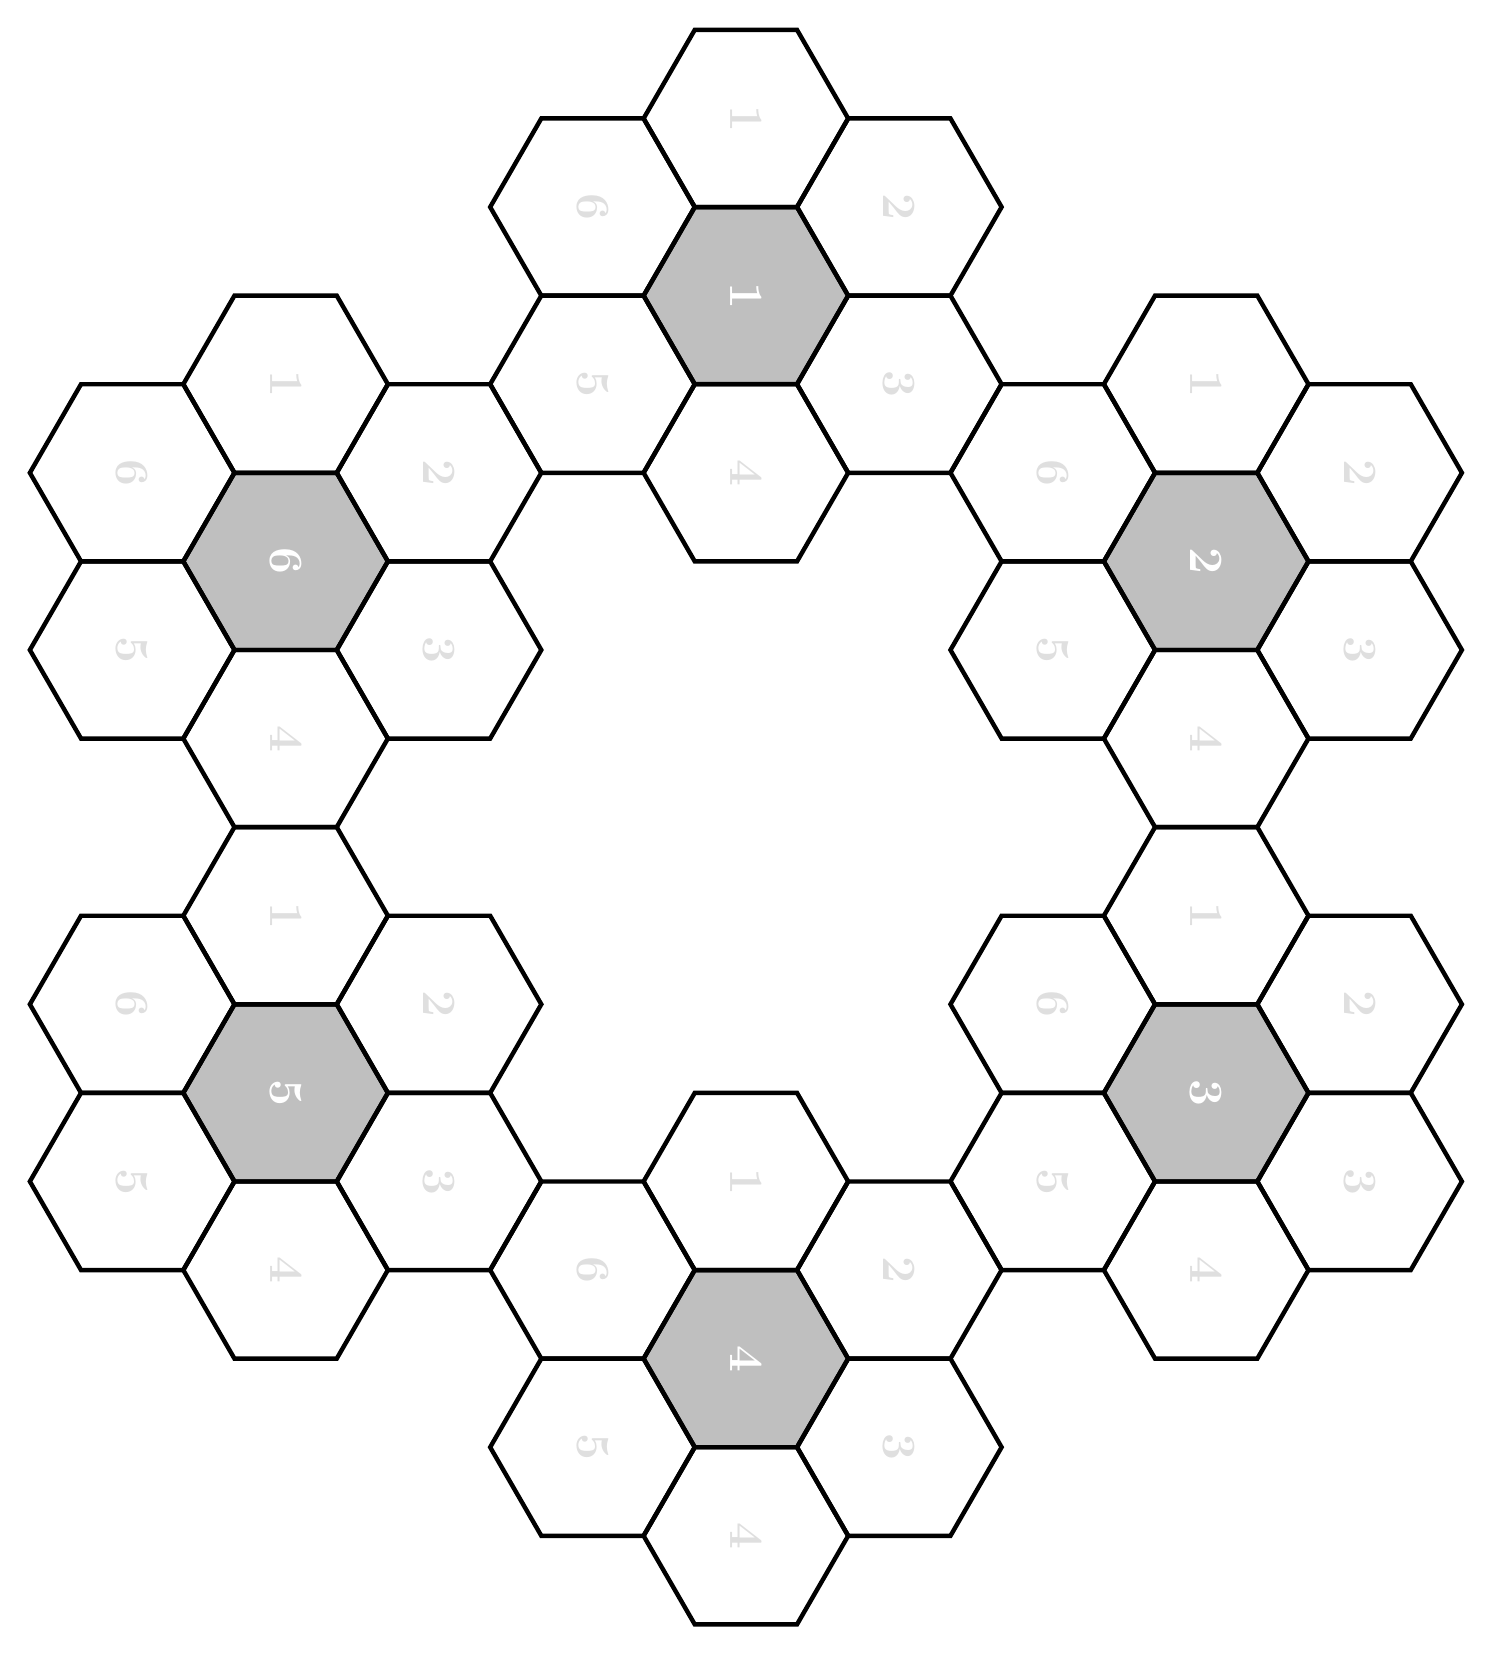
\begin{tikzpicture}
\foreach \i/\j in {30/2, 90/1, 150/6, 210/5, 270/4, 330/3}
	\pic at (\i:6.75cm) {hexflower={\j}};
\end{tikzpicture}
\end{document}